
%%% Local Variables:
%%% mode: latex
%%% TeX-master: t
%%% End:

\chapter{索引相关综述}
\label{cha:related-work}
前文已经提到,近邻查询问题最关键的就是在于如何选取出一个近邻候选集合$S'$。为了快速地删选出近邻候选集,我们通常会先把原始的数据索引起来。依据
不同的索引结构分类,近邻查询的方法一般可以分为基于树结构的索引和基于哈希的索引两大类。
\section{基于树结构的索引}
传统的基于树结构的索引方法有很多,比如 R 树、KD-树、Ball 树等。下面将介绍在 FLANN\cite{muja_flann_2009} 近似近邻搜索中用到的两种树结构的索引方法。
\subsection{随机化 KD-树}
经典的 KD-树会将原始的数据空间不断划分成一棵二叉树。它在低维的空间上检索具有非常高效,但随着维度不断增加,KD-树的检索效率会迅速大幅度降低。因此,许多基于 KD-树改进的工作涌现出来。其中,Silpa-Anan 等人提出的一种随机化的 KD-树\cite{Silpa-AnanH08}的改进方法。原始的 KD-树的方法在空间划分时会选取数据方差最大的维度,在这一维度上将空间一分为二。相比于传统的 KD-树方法,随机化的 KD-树在数据空间切分的时候,并不是固定选择数据方差最大的维度,而是从数据方差比较大前几个维度中随机地选取一个维度进行切分。之所这样处理,是因为在维度较高的情况下(如 50 维),其实数据在许多维度上的方差可能差别不大。通过随机化的选择,这样有更高的概率可以把数据空间中的点切分地比较均匀,从而可以提高近似近邻查询的效率。
\subsection{分层 K-Means 树}
顾名词义,分层 K-Means 树\cite{Nister:2006}是在数据需要切分时,使用 K-Means 聚类的方法将数据切分成 K 份。依照这一方法,在每一层中都使用 K-Means 聚类,当数据的数量少于 K 个时,我们就可以直接将这 K 个节点作为叶子节点。这样,分层 K-Means 树就可以看作是一棵 K 叉树。利用分层 K-Means 树作近似近邻查询的时候,当遍历到某个父亲节点,首先在其子节点当中,选取出一个距离查询数据最近的子节点,然后再优先遍历这个子节点。显然,这样的查询效率是非常高的,能够快速地找到近邻候选集。但是从分层 K-Means 树的建树过程来看,在每一非叶子节点都要执行一次 K-Means 聚类,这种算法不管从时间上还是空间上来计算,代价都是非常大的。
\begin{figure}[H]
  \centering
  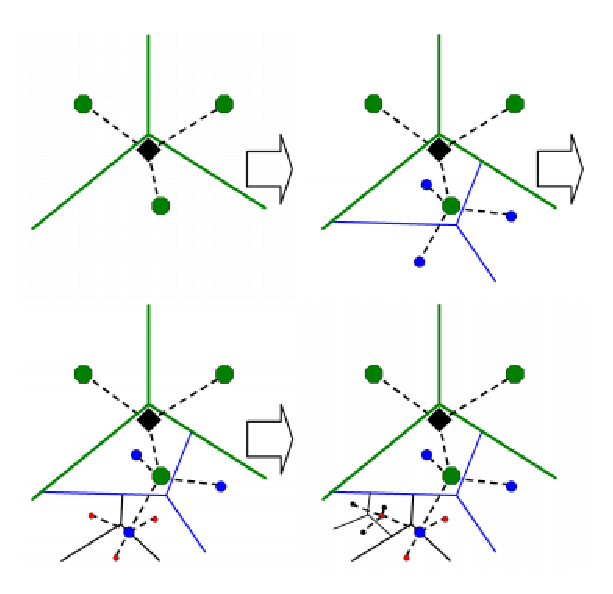
\includegraphics[width=0.5\linewidth]{k-means-tree}
  \caption{聚类中心为 3 的层次K-Means 树建树过程}
  \label{fig:k-means-tree}
  \footnotesize 注:图像来源\cite{Nister:2006}
\end{figure}
\section{基于哈希的索引}
传统基于树结构的索引方法最大的不足就是空间效率不高,随着维度的不断增长,空间代价成倍增长。因此,我们需要对原始的数据集空间进行压缩编码以节省空间。基于哈希的索引方法是将高维的数据压缩成二进制编码的形式,这类方法在大规模的图像、文本、视频等多媒体检索上取得不错的效果。根据哈希函数形式的不同,我们可以粗略地将哈希索引分为两类——汉明嵌入和向量量化。

\subsection{距离度量}
在近似近邻查询中,计算两个数据的距离是不可避免的。在介绍汉明嵌入和向量量化之前,首先介绍一下距离度量方式。

由于哈希的方法将数据进行了编码压缩,我们可能无法直接在原始空间中计算距离。因此这时候可能需要编码空间中距离与原始空间中距离的转换,根据不同转换方式产生两种距离度量方式,分别是对称距离度量(SQD)和非对称距离度量(AQD)。
对于两个数据 $x$ 和 $y$,$x$ 是查询数据,$y$ 是原始数据空间中的一个数据,$q(\cdot)$ 是哈希函数。对称距离的度量方式就是指 $x$ 和 $y$ 之间的距离可以近似地用 $q(x)$ 和 $q(y)$ 之间的距离来表示,用公式表示也就是 $d(x,y) \approx d(q(x),q(y))$。汉明嵌入中用汉明距离\footnote{汉明距离指两个二进制串进行 XOR 操作之后,结果串中 1 的个数。比如,1011001 和 1001101 的汉明距离是 2。}近似原始距离就是一种典型的对称距离的度量方式。非对称距离的度量方式是指 $x$ 和 $y$ 之间的距离用 $x$ 和 $q(y)$ 之间的距离近似表示,也就是 $d(x,y) \approx d(x, q(y))$。$x$ 和 $q(y)$ 之间距离。
\subsection{汉明嵌入}
汉明嵌入的哈希方法就是要寻找一个映射,对于任意的对象$x \in S$都能映射到汉明空间中的二进制串$b(x) \in \{0,1\}^d$。这种映射是保持距离的,也就是在原始空间中距离大小与汉明空间中的距离大小有对应关系。那么,任意两个对象之间的相似度就可以通过其对应二进制串之间的汉明距离来近似计算:
\begin{equation}
sim(x, y)\thickapprox 1 - \frac{2\delta_{Ham}(b(x),b(y))}{d}
\end{equation}
汉明嵌入的哈希方法比较多,谱哈希(Spectral Hashing)\cite{WeissTF08}方法就是其中的代表性方法之一。
\subsubsection{谱哈希}
假设 $\{y_i\}^n_{i=1}$ 是 $n$ 个数据的二进制编码(编码长度为 $k$),邻接矩阵 $W_{n\times n}$用来原始数据点之间的距离。$W_{ij}$ 就表示原始数据空间中第 $i$ 个数据和第 $j$ 个数据之的相似度。原始数据空间中的数据 $i$ 用编码结果用 $y_i \in \{-1,1\}^k$ 表示。为了做到编码保持距离大小对应,也就是说 $W_{i,j}$ 相似度越大,$\lVert y_i - y_j \rVert ^2$ 就应该越小。因此,所有近邻关系中的平均汉明距离可以用$\sum_{ij}W_{ij}\lVert y_i - y_j \rVert ^2$ 表示。那么,我们也就可以得到这个问题的目标函数如下:
\begin{equation}
\label{equ:sh1}
\begin{split}
\mathrm{minimize}: \sum_{ij}W_{ij}\lVert y_i - y_j \rVert ^2 \\
\mathrm{s.t.}: y_i \in \{-1,1\}^k \\
\sum_{i} y_i = 0 \\
\frac{1}{n}\sum_{i}y_iy_i^T = I
\end{split}
\end{equation}

其中 $\sum_{i} y_i = 0$ 约束条件会使编码中 0 和 1 的数量各占一半,$\frac{1}{n}\sum_{i}y_iy_i^T = I $ 则表示任意两个编码之间是不相关的。观察发现,上面的式子是一个 NP 难问题,不能在多项式时间内求解。

我们将公式 \ref{equ:sh1} 进行变形,引入一个 $n\times k$ 大小的矩阵 $Y$,$Y$ 的第 $j$ 列是 $y_j^T$ 。$n\times n$ 的对角矩阵 $D$,其中 $D(i,i)=\sum_{j}W_{ij}$。变换后的公式:
\begin{equation}
\label{equ:sh2}
\begin{split}
\mathrm{minimize}: tr(Y^T(D-W)Y)\\
\mathrm{s.t.}: \sum_{i} Y^T1= 0 \\
Y^TY = I
\end{split}
\end{equation}

相比于公式  \ref{equ:sh1} ,我们去掉了 $Y_{ij}\in \{-1,1\}$ 的约束,$Y_{ij}$ 可以在实数集上取值。这样原来的问题就简化成了求解矩阵 $D-W$ 的 $k$ 个特征向量。对这 $k$ 个特征向量根据正负二值化就可以得到我们原来想要的编码矩阵。
\subsection{向量量化}
向量量化的哈希索引是对原始向量空间进行量化压缩,原始向量$\mathbf{x} \in \mathbb{R}^D$ 通过量化函数 $q$ 被映射到 $q(\mathbf{x}) \in \mathcal{C} = \{\mathbf{c}_i\}$,其中 $i$ 是下标,$\mathbf{c}_i$ 可以称作为码字,而$\mathcal{C}$则被称为码本。 这种映射可以形式化定义成:$\forall \mathbf{x} \in \mathbb{R}^D$,$\exists \mathbf{c}_i \in \mathcal{C} $,$q(\mathbf{x})=\mathbf{c}_i$。整个量化过程中的平均量化误差 $E$ 就可以定义为:
\begin{equation}
E = \frac{1}{n}\sum_{\mathbf{x}}\lVert \mathbf{x} - q(\mathbf{x}) \rVert ^2
\end{equation}

其中$\lVert \cdot \rVert$ 表示欧氏距离,而 $n$ 是数据的总量。对于给定的原始数据集合 $S$,我们的目标是找到一个码本 $\mathcal{C}$ 以及对应量化函数 $q(\mathbf{x})$ 使得量化误差 $E$ 最小。在最小化量化误差过程中,不同的限制条件就对应了不同的量化方法。
\subsubsection{K-Means}
假设有一个包含 $n$ 个 $p$ 维 数据点的集合,$\mathcal{D}\{\mathbf{x}_j\}_{j=1}^n$ , k-means 算法会将这 $n$ 个数据点聚成 $k$ 类,同时用聚类中心来代表每一个聚类的数据。假如矩阵$C \in \mathbb{R}^{p\times k}$的列向量由 $k$ 个聚类构成,每一列都是一个聚类中心,$C=[\mathbf{c}_1,\mathbf{c}_2,\cdots, \mathbf{c}_k]$。k-means 量化的目标函数如下:
\begin{eqnarray}
\mathit{l}_\mathrm{k-means} &=&\sum_{\mathbf{x}\in\mathcal{D}}\min_{i}\lVert \mathbf{x} - \mathbf{c}_i \rVert _2^2 \\
                   &=&\sum_{\mathbf{x}\in\mathcal{D}}\min_{\mathbf{b}\in\mathcal{H}_{1/k}}\lVert \mathbf{x} - C\mathbf{b} \rVert _2^2
\end{eqnarray}

其中$\mathcal{H}_{1/k} = \{\mathbf{b}|\mathbf{b}\in\{0,1\}^k$且$\lVert\mathbf{b}\rVert=1\}$,$\mathbf{b}$ 是一个 1 对 $k$ 编码的二进制向量(包含 1 个 1 ,$k$-1 个 0)。

k-means 量化模型浅显易懂,使用最朴素的近邻查询方法就可以将数据点映射到聚类中心。这种映射过程将每一个原始数据压缩到了 $\log_2k$ 比特的数据,所需要消耗的存储空间随着 $k$ 的线性增长。
\subsubsection{ITQ}
ITQ(Iterative Quantization)\cite{YunchaoGong:2011:IQP:2191740.2191779}的量化方法是在 2011 年的 CVPR 会议上提出,这一方法较之前的哈希方法在准确率上有了显著提升。

ITQ 方法首先是对原始数据集空间进行 PCA 降维,将原始的 $\mathbb{R}^{n\times d}$ 空间降维成 $\mathbb{R}^{n\times c}$ 空间。此时,再
考虑将降维后的数据集进行二进制编码。从降维后的空间中取出$\mathbf{v}\in \mathbb{R}^{c}$,其对应的编码 sgn($\mathbf{v}$) 可以看做事超立方体$\{-1,1\}^c$
中的顶点。此时,欲使整体的量化误差最小,就是要使原始数据与编码后的数据的欧氏距离最小,$\min{\lVert \mathrm{sgn}(\mathbf{v})-\mathbf{v}\rVert ^2}$。
对于编码前的原始数据集我们用 $X \in \mathbb{R}^{n\times d}$ 来表示,经过 PCA 降维后用 $V \in \mathbb{R}^{n\times c}$ 表示,编码后的数据集用 $B \in \{-1,1\}^{n\times c}$ 来表示。
整体量化误差:
\begin{equation}
Q(B, R) = \lVert B - VR \rVert_F ^2
\end{equation}

其中$\lVert \cdot \rVert_F$ 是 Frobenius 范式,而 $R$ 是正交矩阵,作用是对 $V$ 进行旋转对齐。为何要引入这个旋转矩阵 $R$ 呢?从下图(\ref{fig:itq})可以看出,左侧是 PCA 降维后的数据集 $V$,中间是随机旋转后的数据集,右侧是最优化旋转后的数据集 $VR$。右乘一个旋转矩阵 $R$,让待编码的数据绕数据中心进行旋转到合适状态,每个数据点就可以用距离其最近的数据顶点来表示。下图中可以用 $(-1, -1), (-1, 1), (1, 1), (1, -1) $ 这是四个点来表示。此时,所有的数据点到超立方的顶点的距离和最小,也就是量化误差最小。
\begin{figure}[H]
  \centering
  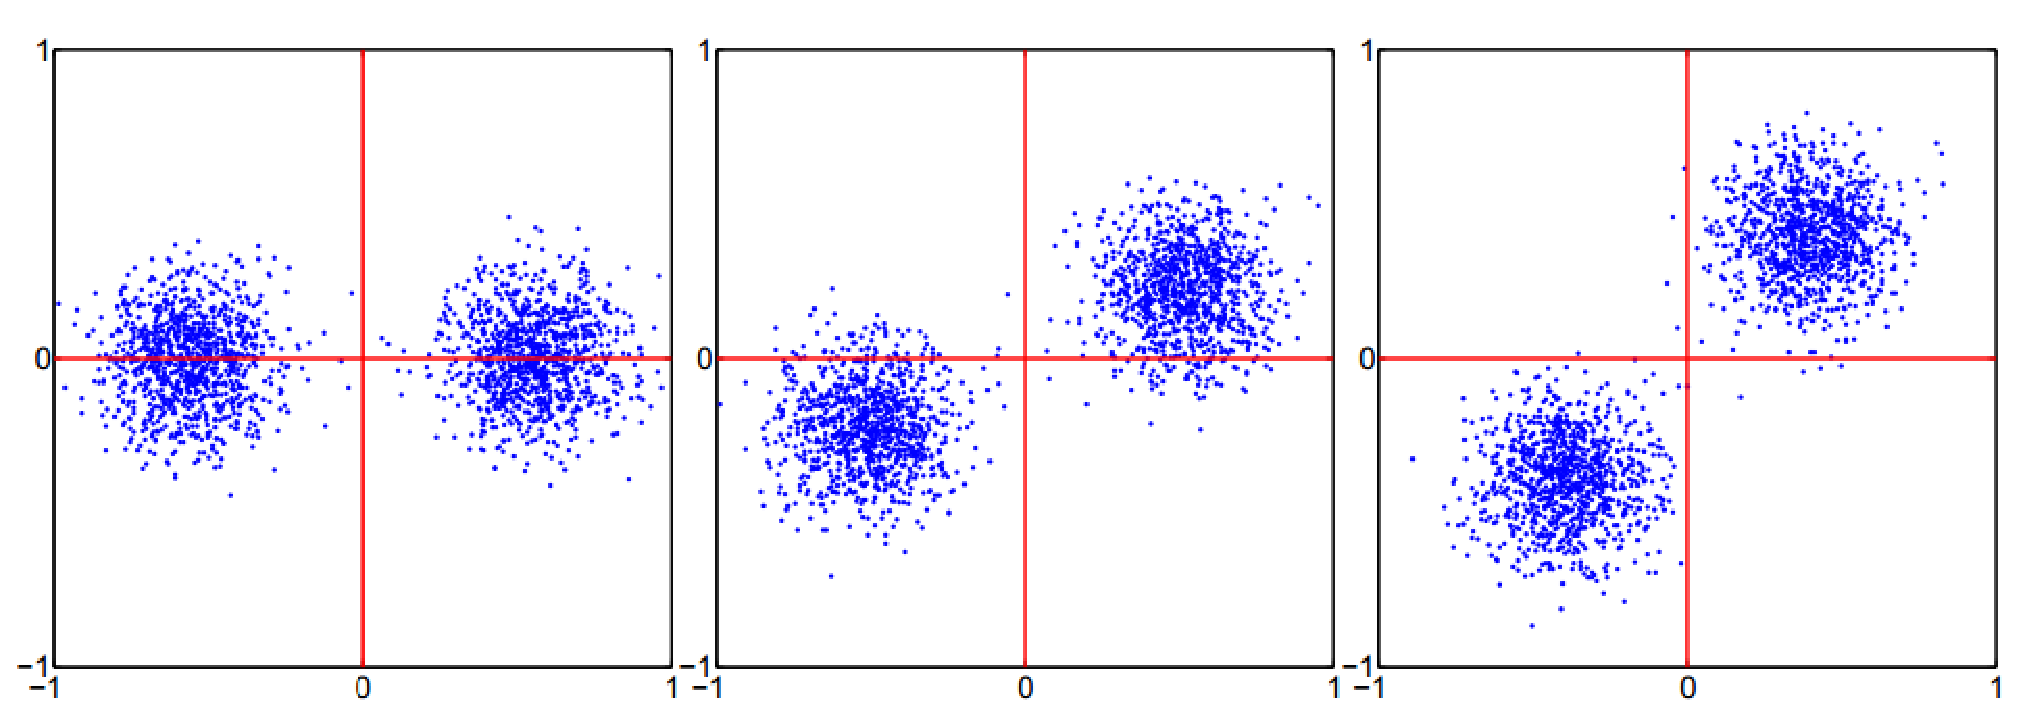
\includegraphics[width=1.0\linewidth]{itq}
  \caption{ITQ 旋转过程}
  \label{fig:itq}
  \footnotesize 注:图像来源\cite{YunchaoGong:2011:IQP:2191740.2191779}
\end{figure}
这样,整个问题的目标函数就变成了$\min \lVert B - VR \rVert_F ^2$。这个公式中有两个未知量,编码后的矩阵 $B$ 和 旋转矩阵 $R$。所以,这个问题的求解要考虑采用交替迭代的方法。先对一个随机生成的矩阵进行 SVD 分解得到一个正交矩阵作为 $R$ 的初始值,此时 $R$ 已知,就可以用$ B= \mathrm{sgn}(VR)$ 来求解 $B$;当 $B$ 已知后,可以对 $B^TV$ 进行 SVD 分解求解 $R$。既然 $R$ 求出,又可以重新一次迭代,固定 $R$ 求 $B$,如此交替迭代就可以求解出该问题。

